\subsection{Experimental methods}
A brief overview of the employed experimental techniques is presented here. Mole fraction time histories of methane ($\mathrm{CH_4}$), acetylene ($\mathrm{C_2H_2}$), and ethylene ($\mathrm{C_2H_4}$) were captured using CW laser absorption at 3.365~$\mu$m, 2.998~$\mu$m, and 10.532~$\mu$m, respectively~\citep{stranic2014laser,pinkowski2019multi,cassady2020thermal}. soot volume fraction was measured using laser light extinction at $\lambda$=633~nm and 1064~nm:
\begin{equation}
f_v=\frac{1}{L}\frac{\mathrm{ln}(I_0/I_t)\lambda}{6\pi E(m)},
\label{eqn:fvext}
\end{equation}
\noindent where $L$=14.12~cm is the absorption path length, equal to the inner diameter of the shock tube. $\lambda$ is the absorption wavelength, and $I_0$ and $I_t$ are the incident and transmitted intensities, respectively. Table~\ref{tab:TP5_exec_tests} indicates the conditions of the shock-tube tests with 1800~K$<$T$_5$$<$2400~K and P$_5$=4.5$\pm$0.5~atm. $f_v$ was determined from the measured extinction at 633~nm and 1064~nm, considering the reported variability of $E(m)$ in the literature, ranging from 0.174~\citep{lee1981optical} to 0.26~\citep{dalzell1969optical} for 633~nm and from 0.2 to 0.3 for 1064~nm~\citep{bladh2011optical}.

Additionally, soot samples were collected onto imaging stubs mounted in the shock-tube endwall. Samples were extracted from the interior surface of the shock tube endwall after each experiment to allow for imaging and analysis of the particulates. TEM images were recorded with a FEI Tecnai G2 F20 X-TWIN microscope and Gatan SC200 camera for all test cases. Primary particle diameter, $d_p$, was obtained by visually identifying the smallest circumscribed circle enclosing each primary particle in the TEM images and calculating the arithmetic and geometric means. A minimum of 200 primary particles were measured for each condition. Fig.~\ref{fig:2203K_sample_tem} depicts representative TEM images collected for the test at T$_5$=2203~K, with identified primary particles shown as superimposed red circles.


\renewcommand{\arraystretch}{1.5}
\begin{table}[!t]
	\centering
	\caption{The post-reflected-shock pressure (P$_5$) and temperature (T$_5$) of the executed shock-tube tests.}
	\label{tab:TP5_exec_tests}
    \begin{tabular}{llllllll}
    \hline
     & (1)  & (2)  & (3)  & (4)  & (5)  & (6)  & (7)  \\ \hline
    T$_5$~[K]   & 1875 & 1984 & 2132 & 2203 & 2247 & 2322 & 2355 \\ \hline
    P$_5$~[atm] & 4.45 & 4.30 & 4.17 & 4.90 & 4.51 & 4.55 & 4.64 \\ \hline
    \end{tabular}
\end{table}


\begin{figure}[!t]
	\centering
	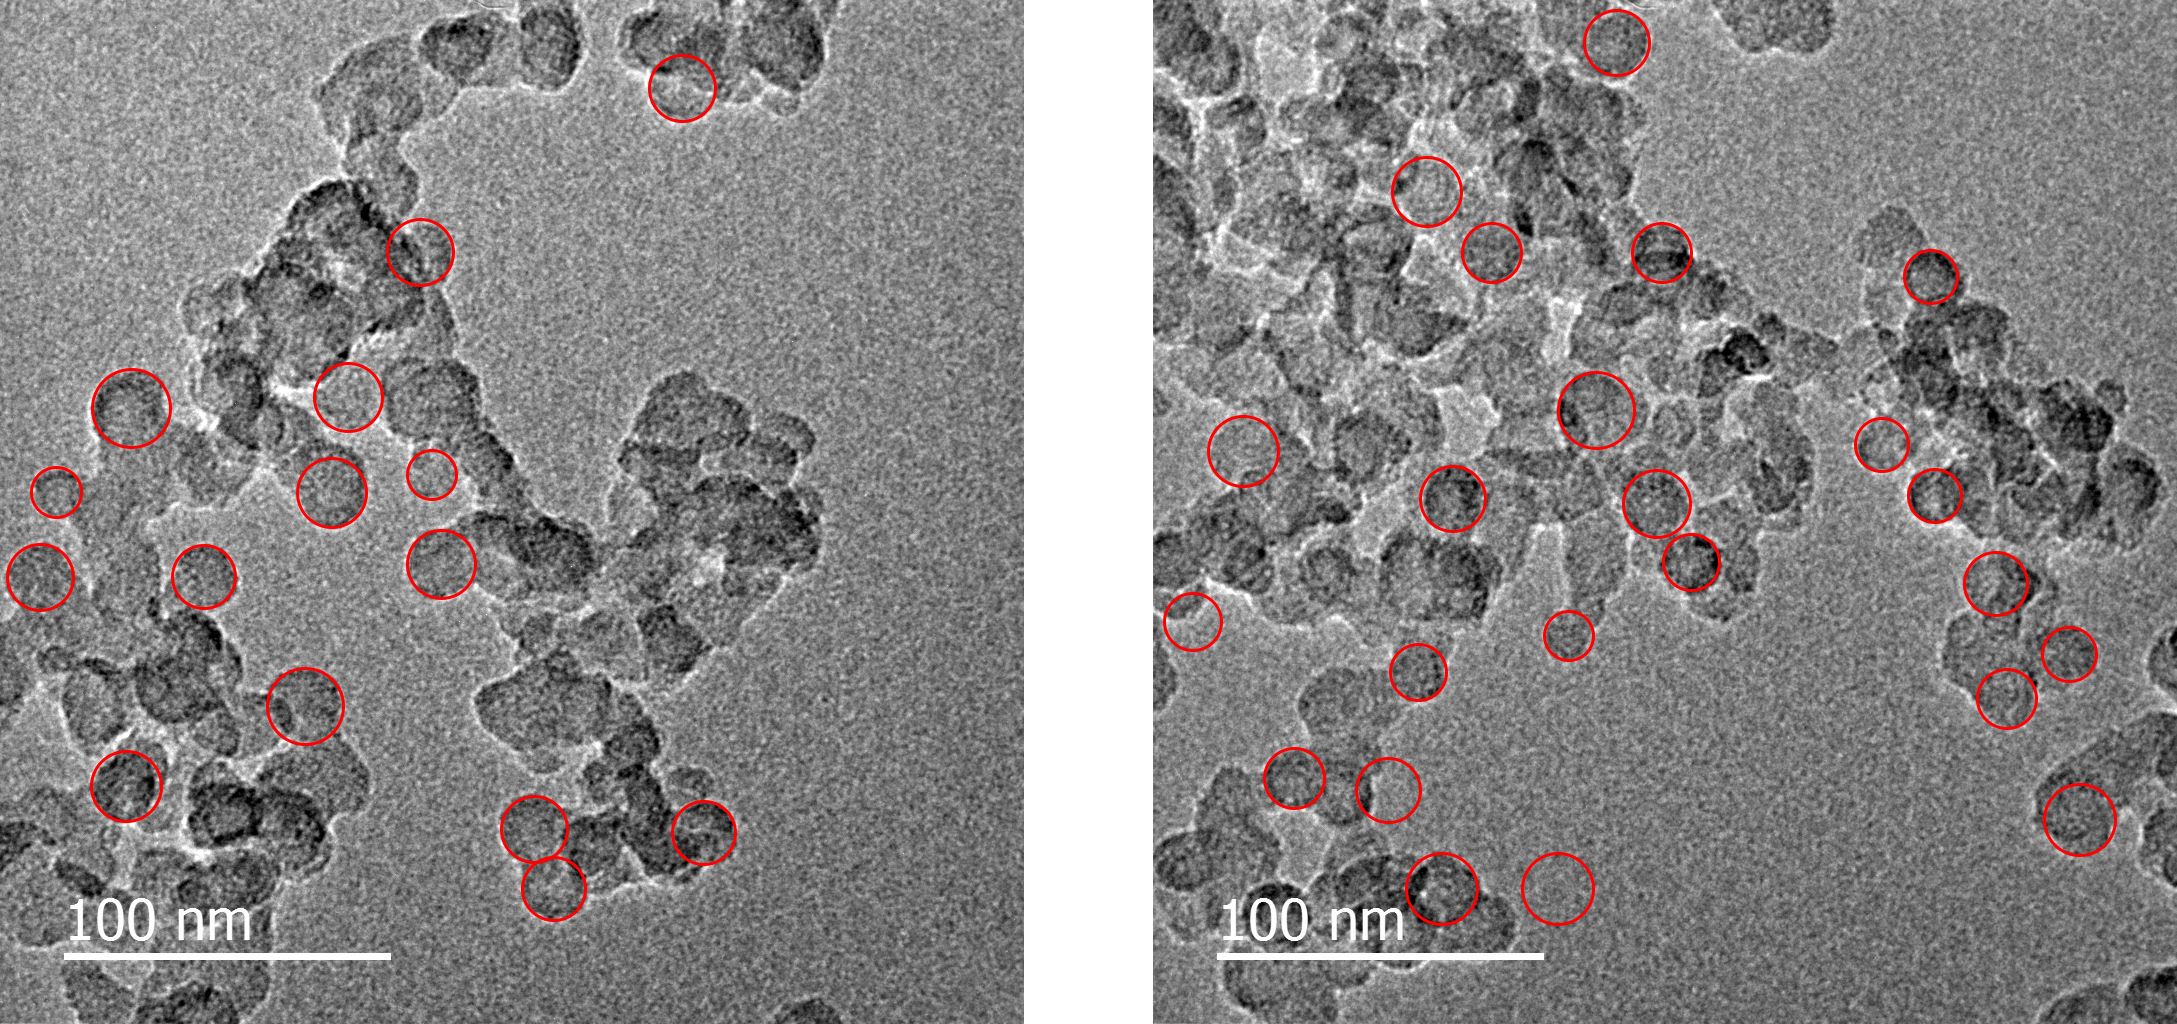
\includegraphics[width=0.75\textwidth]{Figures/Results/Paper3/2203K_TEM_detected_sample_two.jpg}
	\caption{Samples of TEM images collected for T$_5$=2203~K. Red circles represent the identified primary particles used to measure $d_p$.}
	\label{fig:2203K_sample_tem} 
\end{figure}